% defer/rcuAPI.tex

\subsection{RCU Linux-Kernel API}
\label{sec:defer:RCU Linux-Kernel API}
\OriginallyPublished{Section}{sec:defer:RCU Linux-Kernel API}{RCU Linux-Kernel API}{Linux Weekly News}{PaulEMcKenney2008WhatIsRCUAPI}

This section looks at RCU from the viewpoint of its Linux-kernel API.
Section~\ref{sec:defer:RCU has a Family of Wait-to-Finish APIs}
presents RCU's wait-to-finish APIs, and
Section~\ref{sec:defer:RCU has Publish-Subscribe and Version-Maintenance APIs}
presents RCU's publish-subscribe and version-maintenance APIs.
Finally,
Section~\ref{sec:defer:So, What is RCU Really?}
presents concluding remarks.

\subsubsection{RCU has a Family of Wait-to-Finish APIs}
\label{sec:defer:RCU has a Family of Wait-to-Finish APIs}

\begin{table*}[p]
\begin{center}
\scriptsize
\begin{tabular}{p{1.1in}|p{1.0in}|p{1.1in}|p{1.0in}|p{1.0in}}
Attribute &
    RCU Classic &
	RCU BH &
	    RCU Sched &
		Realtime RCU \\
\hline
\hline
Purpose &
    Original &
	Prevent DDoS attacks &
	    { \raggedright Wait for preempt-disable regions,
	      hardirqs, \& NMIs } &
	        Realtime response \\
\hline
Availability &
    2.5.43 &
	2.6.9 &
	    2.6.12 &
	        2.6.26 \\
\hline
Read-side primitives &
    { \raggedright
      \url{rcu_read_lock()}~! \\
      \url{rcu_read_unlock()}~! } &
	{ \raggedright
	  \url{rcu_read_lock_bh()} \\
	  \url{rcu_read_unlock_bh()} } &
	    { \raggedright
	      \url{preempt_disable()} \\
	      \url{preempt_enable()} \\
	      (and friends) } &
	        { \raggedright
		  \url{rcu_read_lock()} \\
		  \url{rcu_read_unlock()} } \\
\hline
{ Update-side primitives (synchronous) } &
    { \url{synchronize_rcu()} \url{synchronize_net()} } &
	&
	    \url{synchronize_sched()} &
	        { \url{synchronize_rcu()} \url{synchronize_net()} } \\
\hline
{ Update-side primitives (asynchronous/callback) } &
    \url{call_rcu()} ! &
	\url{call_rcu_bh()} &
	    \url{call_rcu_sched()} &
	        \url{call_rcu()} \\
\hline
{ Update-side primitives (wait for callbacks) } &
    \url{rcu_barrier()} &
	\url{rcu_barrier_bh()} &
	    \url{rcu_barrier_sched()} &
	        \url{rcu_barrier()} \\
\hline
Type-safe memory &
    \url{SLAB_DESTROY_BY_RCU} &
	&
	    &
	        \url{SLAB_DESTROY_BY_RCU} \\
\hline
Read side constraints &
    No blocking &
	No irq enabling &
	    No blocking &
	        Only preemption and lock acquisition \\
\hline
Read side overhead &
    Preempt disable/enable (free on non-PREEMPT) &
	BH disable/enable &
	    Preempt disable/enable (free on non-PREEMPT) &
	        Simple instructions, irq disable/enable \\
\hline
Asynchronous update-side overhead &
    sub-microsecond &
	sub-microsecond &
	    &
	        sub-microsecond \\
\hline
Grace-period latency &
    10s of milliseconds &
	10s of milliseconds &
	    10s of milliseconds &
	        10s of milliseconds \\
\hline
Non-\url{PREEMPT_RT} implementation &
    RCU Classic &
	RCU BH &
	    RCU Classic &
	        Preemptible RCU \\
\hline
\url{PREEMPT_RT} implementation &
    Preemptible RCU &
	Realtime RCU &
	    Forced Schedule on all CPUs &
	        Realtime RCU \\
\end{tabular}
\end{center}
\caption{RCU Wait-to-Finish APIs}
\label{tab:defer:RCU Wait-to-Finish APIs}
\end{table*}

\begin{table*}[p]
\begin{center}
\scriptsize
\begin{tabular}{p{1.1in}|p{1.5in}|p{1.5in}}
Attribute &
    SRCU &
	QRCU \\
\hline
\hline
Purpose &
    Sleeping readers &
	Sleeping readers and fast grace periods \\
\hline
Availability &
    2.6.19 &
	\\
\hline
Read-side primitives &
    { \raggedright
      \url{srcu_read_lock()} \\
      \url{srcu_read_unlock()} } &
	{ \raggedright
	  \url{qrcu_read_lock()} \\
	  \url{qrcu_read_unlock()} } \\
\hline
{ Update-side primitives (synchronous) } &
    \url{synchronize_srcu()} &
	\url{synchronize_qrcu()} \\
\hline
{ Update-side primitives (asynchronous/callback) } &
    N/A &
	N/A \\
\hline
{ Update-side primitives (wait for callbacks) } &
    N/A &
	N/A \\
\hline
Type-safe memory &
    &
	\\
\hline
Read side constraints &
    No \url{synchronize_srcu()} &
	No \url{synchronize_qrcu()} \\
\hline
Read side overhead &
    Simple instructions, preempt disable/enable &
	Atomic increment and decrement of shared variable \\
\hline
Asynchronous update-side overhead &
    N/A &
	N/A \\
\hline
Grace-period latency &
    10s of milliseconds &
	10s of \emph{nanoseconds} in absence of readers \\
\hline
Non-\url{PREEMPT_RT} implementation &
    SRCU &
	N/A \\
\hline
\url{PREEMPT_RT} implementation &
    SRCU &
	N/A \\
\end{tabular}
\end{center}
\caption{Sleepable RCU Wait-to-Finish APIs}
\label{tab:defer:Sleepable RCU Wait-to-Finish APIs}
\end{table*}

The most straightforward answer to ``what is RCU'' is that RCU is
an API used in the Linux kernel, as summarized by
Tables~\ref{tab:defer:RCU Wait-to-Finish APIs} and
\ref{tab:defer:Sleepable RCU Wait-to-Finish APIs},
which shows the wait-for-RCU-readers portions of the non-sleepable and
sleepable APIs, respectively,
and by
Table~\ref{tab:defer:RCU Publish-Subscribe and Version Maintenance APIs},
which shows the publish/subscribe portions of the API.

If you are new to RCU, you might consider focusing on just one
of the columns in
Table~\ref{tab:defer:RCU Wait-to-Finish APIs},
each of which summarizes one member of the Linux kernel's RCU API family..
For example, if you are primarily interested in understanding how RCU
is used in the Linux kernel, ``RCU Classic'' would be the place to start,
as it is used most frequently.
On the other hand, if you want to understand RCU for its own sake,
``SRCU'' has the simplest API.
You can always come back for the other columns later.

If you are already familiar with RCU, these tables can
serve as a useful reference.

\QuickQuiz{}
	Why do some of the cells in
	Table~\ref{tab:defer:RCU Wait-to-Finish APIs}
	have exclamation marks (``!'')?
\QuickQuizAnswer{
	The API members with exclamation marks (\url{rcu_read_lock()},
	\url{rcu_read_unlock()}, and \url{call_rcu()}) were the
	only members of the Linux RCU API that Paul E. McKenney was aware
	of back in the mid-90s.
	During this timeframe, he was under the mistaken impression that
	he knew all that there is to know about RCU.
} \QuickQuizEnd

The ``RCU Classic'' column corresponds to the original RCU implementation,
in which RCU read-side critical sections are delimited by
\url{rcu_read_lock()} and \url{rcu_read_unlock()}, which
may be nested.
The corresponding synchronous update-side primitives,
\url{synchronize_rcu()}, along with its synonym
\url{synchronize_net()}, wait for any currently executing
RCU read-side critical sections to complete.
The length of this wait is known as a ``grace period''.
The asynchronous update-side primitive, \url{call_rcu()},
invokes a specified function with a specified argument after a
subsequent grace period.
For example, \url{call_rcu(p,f);} will result in
the ``RCU callback'' \url{f(p)}
being invoked after a subsequent grace period.
There are situations,
such as when unloading a Linux-kernel module that uses \url{call_rcu()},
when it is necessary to wait for all
outstanding RCU callbacks to complete~\cite{PaulEMcKenney2007rcubarrier}.
The \url{rcu_barrier()} primitive does this job.
Note that the more recent hierarchical
RCU~\cite{PaulEMcKenney2008HierarchicalRCU}
implementation described in
Sections~\ref{app:rcuimpl:rcutree:Hierarchical RCU Overview} and
\ref{app:rcuimpl:rcutreewt:Hierarchical RCU Code Walkthrough}
also adheres to ``RCU Classic'' semantics.

Finally, RCU may be used to provide
type-safe memory~\cite{Cheriton96a}, as described in
Section~\ref{sec:deferRCU is a Way of Providing Type-Safe Memory}.
In the context of RCU, type-safe memory guarantees that a given
data element will not change type during any RCU read-side critical section
that accesses it.
To make use of RCU-based type-safe memory, pass
\url{SLAB_DESTROY_BY_RCU} to
\url{kmem_cache_create()}.
It is important to note that \url{SLAB_DESTROY_BY_RCU} will
\emph{in no way}
prevent \url{kmem_cache_alloc()} from immediately reallocating
memory that was just now freed via \url{kmem_cache_free()}!
In fact, the \url{SLAB_DESTROY_BY_RCU}-protected data structure
just returned by \url{rcu_dereference} might be freed and reallocated
an arbitrarily large number of times, even when under the protection
of \url{rcu_read_lock()}.
Instead, \url{SLAB_DESTROY_BY_RCU} operates by preventing
\url{kmem_cache_free()}
from returning a completely freed-up slab of data structures
to the system until after an RCU grace period elapses.
In short, although the data element might be freed and reallocated arbitrarily
often, at least its type will remain the same.

\QuickQuiz{}
	How do you prevent a huge number of RCU read-side critical
	sections from indefinitely blocking a \url{synchronize_rcu()}
	invocation?
\QuickQuizAnswer{
	There is no need to do anything to prevent RCU read-side
	critical sections from indefinitely blocking a
	\url{synchronize_rcu()} invocation, because the
	\url{synchronize_rcu()} invocation need wait only for
	\emph{pre-existing} RCU read-side critical sections.
	So as long as each RCU read-side critical section is
	of finite duration, there should be no problem.
} \QuickQuizEnd

\QuickQuiz{}
	The \url{synchronize_rcu()} API waits for all pre-existing
	interrupt handlers to complete, right?
\QuickQuizAnswer{
	Absolutely not!!!
	And especially not when using preemptible RCU!
	You instead want \url{synchronize_irq()}.
	Alternatively, you can place calls to \url{rcu_read_lock()}
	and \url{rcu_read_unlock()} in the specific interrupt handlers that
	you want \url{synchronize_rcu()} to wait for.
} \QuickQuizEnd

In the ``RCU BH'' column, \url{rcu_read_lock_bh()} and
\url{rcu_read_unlock_bh()} delimit RCU read-side critical
sections, and \url{call_rcu_bh()} invokes the specified
function and argument after a subsequent grace period.
Note that RCU BH does not have a synchronous \url{synchronize_rcu_bh()}
interface,
though one could easily be added if required.

\QuickQuiz{}
	What happens if you mix and match?
	For example, suppose you use \url{rcu_read_lock()} and
	\url{rcu_read_unlock()} to delimit RCU read-side critical
	sections, but then use \url{call_rcu_bh()} to post an
	RCU callback?
\QuickQuizAnswer{
	If there happened to be no RCU read-side critical
	sections delimited by \url{rcu_read_lock_bh()} and
	\url{rcu_read_unlock_bh()} at the time \url{call_rcu_bh()}
	was invoked, RCU would be within its rights to invoke the callback
	immediately, possibly freeing a data structure still being used by
	the RCU read-side critical section!
	This is not merely a theoretical possibility: a long-running RCU
	read-side critical section delimited by \url{rcu_read_lock()}
	and \url{rcu_read_unlock()} is vulnerable to this failure mode.

	This vulnerability disappears in -rt kernels, where
	RCU Classic and RCU BH both map onto a common implementation.
} \QuickQuizEnd

\QuickQuiz{}
	Hardware interrupt handlers can be thought of as being
	under the protection of an implicit \url{rcu_read_lock_bh()},
	right?
\QuickQuizAnswer{
	Absolutely not!!!
	And especially not when using preemptible RCU!
	If you need to access ``rcu\_bh''-protected data structures
	in an interrupt handler, you need to provide explicit calls to
	\url{rcu_read_lock_bh()} and \url{rcu_read_unlock_bh()}.
} \QuickQuizEnd

In the ``RCU Sched'' column, anything that disables preemption
acts as an RCU read-side critical section, and \url{synchronize_sched()}
waits for the corresponding RCU grace period.
This RCU API family was added in the 2.6.12 kernel, which split the
old \url{synchronize_kernel()} API into the current
\url{synchronize_rcu()} (for RCU Classic) and
\url{synchronize_sched()} (for RCU Sched).
Note that RCU Sched did not originally have an asynchronous
\url{call_rcu_sched()} interface, but one was added in 2.6.26.
In accordance with the quasi-minimalist philosophy of the Linux
community, APIs are added on an as-needed basis.

\QuickQuiz{}
	What happens if you mix and match RCU Classic and RCU Sched?
\QuickQuizAnswer{
	In a non-\url{PREEMPT} or a \url{PREEMPT} kernel, mixing these
	two works "by accident" because in those kernel builds, RCU Classic
	and RCU Sched map to the same implementation.
	However, this mixture is fatal in \url{PREEMPT_RT} builds using the -rt
	patchset, due to the fact that Realtime RCU's read-side critical
	sections can be preempted, which would permit
	\url{synchronize_sched()} to return before the
	RCU read-side critical section reached its \url{rcu_read_unlock()}
	call.
	This could in turn result in a data structure being freed before the
	read-side critical section was finished with it,
	which could in turn greatly increase the actuarial risk experienced
	by your kernel.

	In fact, the split between RCU Classic and RCU Sched was inspired
	by the need for preemptible RCU read-side critical sections.
} \QuickQuizEnd

\QuickQuiz{}
	In general, you cannot rely on \url{synchronize_sched()} to
	wait for all pre-existing interrupt handlers,
	right?
\QuickQuizAnswer{
	That is correct!
	Because -rt Linux uses threaded interrupt handlers, there can
	be context switches in the middle of an interrupt handler.
	Because \url{synchronize_sched()} waits only until each
	CPU has passed through a context switch, it can return
	before a given interrupt handler completes.

	If you need to wait for a given interrupt handler to complete,
	you should instead use \url{synchronize_irq()} or place
	explicit RCU read-side critical sections in the interrupt
	handlers that you wish to wait on.
} \QuickQuizEnd

The ``Realtime RCU'' column has the same API as does
RCU Classic, the only difference being that RCU read-side critical
sections may be preempted and may block while acquiring spinlocks.
The design of Realtime RCU is described
elsewhere~\cite{PaulEMcKenney2007PreemptibleRCU}.

\QuickQuiz{}
	Why do both SRCU and QRCU lack asynchronous \url{call_srcu()}
	or \url{call_qrcu()} interfaces?
\QuickQuizAnswer{
	Given an asynchronous interface, a single task
	could register an arbitrarily large number of SRCU or QRCU callbacks,
	thereby consuming an arbitrarily large quantity of memory.
	In contrast, given the current synchronous
	\url{synchronize_srcu()} and \url{synchronize_qrcu()}
	interfaces, a given task must finish waiting for a given grace period
	before it can start waiting for the next one.
} \QuickQuizEnd

The ``SRCU'' column in
Table~\ref{tab:defer:Sleepable RCU Wait-to-Finish APIs}
displays a specialized RCU API that permits
general sleeping in RCU read-side critical sections
(see Appendix~\ref{app:rcuimpl:Sleepable RCU Implementation} for more details).
Of course,
use of \url{synchronize_srcu()} in an SRCU read-side
critical section can result in
self-deadlock, so should be avoided.
SRCU differs from earlier RCU implementations in that the caller
allocates an \url{srcu_struct} for each distinct SRCU
usage.
This approach prevents SRCU read-side critical sections from blocking
unrelated \url{synchronize_srcu()} invocations.
In addition, in this variant of RCU, \url{srcu_read_lock()}
returns a value that must be passed into the corresponding
\url{srcu_read_unlock()}.

The ``QRCU'' column presents an RCU implementation with the same
API structure as SRCU, but optimized for extremely low-latency
grace periods in absence of readers, as described
elsewhere~\cite{PaulEMcKenney2007QRCUspin}.
As with SRCU, use of \url{synchronize_qrcu()} in a QRCU read-side
critical section can result in
self-deadlock, so should be avoided.
Although QRCU has not yet been accepted into the Linux kernel, it
is worth mentioning given that it is the only kernel-level
RCU implementation
that can boast deep sub-microsecond grace-period latencies.

\QuickQuiz{}
	Under what conditions can \url{synchronize_srcu()} be safely
	used within an SRCU read-side critical section?
\QuickQuizAnswer{
	In principle, you can use
	\url{synchronize_srcu()} with a given \url{srcu_struct}
	within an SRCU read-side critical section that uses some other
	\url{srcu_struct}.
	In practice, however, doing this is almost certainly a bad idea.
	In particular, the code shown in
	Figure~\ref{fig:defer:Multistage SRCU Deadlocks}
	could still result in deadlock.

\begin{figure}[htbp]
{ \centering
\begin{verbatim}
  1 idx = srcu_read_lock(&ssa);
  2 synchronize_srcu(&ssb);
  3 srcu_read_unlock(&ssa, idx);
  4
  5 /* . . . */
  6
  7 idx = srcu_read_lock(&ssb);
  8 synchronize_srcu(&ssa);
  9 srcu_read_unlock(&ssb, idx);
\end{verbatim}
}
\caption{Multistage SRCU Deadlocks}
\label{fig:defer:Multistage SRCU Deadlocks}
\end{figure}

} \QuickQuizEnd

The Linux kernel currently has a surprising number of RCU APIs and
implementations.
There is some hope of reducing this number, evidenced by the fact
that a given build of the Linux kernel currently has at most
three implementations behind four APIs (given that RCU Classic
and Realtime RCU share the same API).
However, careful inspection and analysis will be required, just as
would be required in order to eliminate one of the many locking APIs.

The various RCU APIs are distinguished by the forward-progress
guarantees that their RCU read-side critical sections must provide,
and also by their scope, as follows:

\begin{enumerate}
\item	RCU BH: read-side critical sections
	must guarantee forward progress against everything except for
	NMI and IRQ handlers, but not including softirq handlers.
	RCU BH is global in scope.
\item	RCU Sched: read-side critical sections must guarantee forward
	progress against everything except for NMI and IRQ handlers,
	including softirq handlers.
	RCU Sched is global in scope.
\item	RCU (both classic and real-time): read-side critical sections
	must guarantee forward progress against everything except for
	NMI handlers, IRQ handlers, softirq handlers, and (in the
	real-time case) higher-priority real-time tasks.
	RCU is global in scope.
\item	SRCU and QRCU: read-side critical sections need not guarantee
	forward progress unless some other task is waiting for the
	corresponding grace period to complete, in which case these
	read-side critical sections should complete in no more than
	a few seconds (and preferably much more quickly).\footnote{
		Thanks to James Bottomley for urging me to this
		formulation, as opposed to simply saying that
		there are no forward-progress guarantees.}
	SRCU's and QRCU's scope is defined by the use of the corresponding
	\url{srcu_struct} or \url{qrcu_struct}, respectively.
\end{enumerate}

In other words, SRCU and QRCU compensate for their extremely weak
forward-progress guarantees by permitting the developer to restrict
their scope.

\subsubsection{RCU has Publish-Subscribe and Version-Maintenance APIs}
\label{sec:defer:RCU has Publish-Subscribe and Version-Maintenance APIs}

Fortunately, the RCU publish-subscribe and version-maintenance
primitives shown in the following
table apply to all of the variants of RCU discussed above.
This commonality can in some cases allow more code to be shared,
which certainly reduces the API proliferation that would otherwise
occur.
The original purpose of the RCU publish-subscribe APIs was to
bury memory barriers into these APIs, so that Linux kernel
programmers could use RCU without needing to become expert on
the memory-ordering models of each of the 20+ CPU families
that Linux supports~\cite{Spraul01}.

\begin{table*}[tb]
\begin{center}
% \scriptsize
\begin{tabular}{p{1.1in}|p{1.9in}|p{0.7in}|p{1.3in}}
Category &
	Primitives &
		Availability &
			Overhead \\
\hline
\hline
List traversal &
	\url{list_for_each_entry_rcu()} &
		2.5.59 &
			{ \raggedright
			  Simple instructions (memory barrier on Alpha) } \\
\hline
List update &
	\url{list_add_rcu()} &
		2.5.44 &
			Memory barrier \\
&
	\url{list_add_tail_rcu()} &
		2.5.44 &
			Memory barrier \\
&
	\url{list_del_rcu()} &
		2.5.44 &
			Simple instructions \\
&
	\url{list_replace_rcu()} &
		2.6.9 &
			Memory barrier \\
&
	\url{list_splice_init_rcu()} &
		2.6.21 &
			Grace-period latency \\
\hline
Hlist traversal &
	\url{hlist_for_each_entry_rcu()} &
		2.6.8 &
			{ \raggedright
			  Simple instructions (memory barrier on Alpha) } \\
&
	\url{hlist_add_after_rcu()} &
		2.6.14 &
			Memory barrier \\
&
	\url{hlist_add_before_rcu()} &
		2.6.14 &
			Memory barrier \\
&
	\url{hlist_add_head_rcu()} &
		2.5.64 &
			Memory barrier \\
&
	\url{hlist_del_rcu()} &
		2.5.64 &
			Simple instructions \\
&
	\url{hlist_replace_rcu()} &
		2.6.15 &
			Memory barrier \\
\hline
Pointer traversal &
	\url{rcu_dereference()} &
		2.6.9 &
			{ \raggedright
			  Simple instructions (memory barrier on Alpha) } \\
\hline
Pointer update &
	\url{rcu_assign_pointer()} &
		2.6.10 &
			Memory barrier \\
\end{tabular}
\end{center}
\caption{RCU Publish-Subscribe and Version Maintenance APIs}
\label{tab:defer:RCU Publish-Subscribe and Version Maintenance APIs}
\end{table*}

The first pair of categories operate on Linux
\url{struct}~\url{list_head} lists, which are circular, doubly-linked
lists.
The \url{list_for_each_entry_rcu()} primitive traverses an
RCU-protected list in a type-safe manner, while also enforcing
memory ordering for situations where a new list element is inserted
into the list concurrently with traversal.
On non-Alpha platforms, this primitive incurs little or no performance
penalty compared to \url{list_for_each_entry()}.
The \url{list_add_rcu()}, \url{list_add_tail_rcu()},
and \url{list_replace_rcu()} primitives are analogous to
their non-RCU counterparts, but incur the overhead of an additional
memory barrier on weakly-ordered machines.
The \url{list_del_rcu()} primitive is also analogous to its
non-RCU counterpart, but oddly enough is very slightly faster due to the
fact that it poisons only the \url{prev} pointer rather than
both the \url{prev} and \url{next} pointers as
\url{list_del()} must do.
Finally, the \url{list_splice_init_rcu()} primitive is similar
to its non-RCU counterpart, but incurs a full grace-period latency.
The purpose of this grace period is to allow RCU readers to finish
their traversal of the source list before completely disconnecting
it from the list header -- failure to do this could prevent such
readers from ever terminating their traversal.

\QuickQuiz{}
	Why doesn't \url{list_del_rcu()} poison both the \url{next}
	and \url{prev} pointers?
\QuickQuizAnswer{
	Poisoning the \url{next} pointer would interfere
	with concurrent RCU readers, who must use this pointer.
	However, RCU readers are forbidden from using the \url{prev}
	pointer, so it may safely be poisoned.
} \QuickQuizEnd

The second pair of categories operate on Linux's
\url{struct}~\url{hlist_head}, which is a linear linked list.
One advantage of \url{struct}~\url{hlist_head} over
\url{struct}~\url{list_head} is that the former requires only
a single-pointer list header, which can save significant memory in
large hash tables.
The \url{struct}~\url{hlist_head} primitives in the table
relate to their non-RCU counterparts in much the same way as do the
\url{struct}~\url{list_head} primitives.

The final pair of categories operate directly on pointers, and
are useful for creating RCU-protected non-list data structures,
such as RCU-protected arrays and trees.
The \url{rcu_assign_pointer()} primitive ensures that any
prior initialization remains ordered before the assignment to the
pointer on weakly ordered machines.
Similarly, the \url{rcu_dereference()} primitive ensures that subsequent
code dereferencing the pointer will see the effects of initialization code
prior to the corresponding \url{rcu_assign_pointer()} on
Alpha CPUs.
On non-Alpha CPUs, \url{rcu_dereference()} documents which pointer
dereferences are protected by RCU.

\QuickQuiz{}
	Normally, any pointer subject to \url{rcu_dereference()} \emph{must}
	always be updated using \url{rcu_assign_pointer()}.
	What is an exception to this rule?
\QuickQuizAnswer{
	One such exception is when a multi-element linked
	data structure is initialized as a unit while inaccessible to other
	CPUs, and then a single \url{rcu_assign_pointer()} is used
	to plant a global pointer to this data structure.
	The initialization-time pointer assignments need not use
	\url{rcu_assign_pointer()}, though any such assignments that
	happen after the structure is globally visible \url{must} use
	\url{rcu_assign_pointer()}.

	However, unless this initialization code is on an impressively hot
	code-path, it is probably wise to use \url{rcu_assign_pointer()}
	anyway, even though it is in theory unnecessary.
	It is all too easy for a "minor" change to invalidate your cherished
	assumptions about the initialization happening privately.
} \QuickQuizEnd

\QuickQuiz{}
	Are there any downsides to the fact that these traversal and update
	primitives can be used with any of the RCU API family members?
\QuickQuizAnswer{
	It can sometimes be difficult for automated
	code checkers such as ``sparse'' (or indeed for human beings) to
	work out which type of RCU read-side critical section a given
	RCU traversal primitive corresponds to.
	For example, consider the code shown in
	Figure~\ref{fig:defer:Diverse RCU Read-Side Nesting}.

\begin{figure}[htbp]
{ \centering
\begin{verbatim}
  1 rcu_read_lock();
  2 preempt_disable();
  3 p = rcu_dereference(global_pointer);
  4
  5 /* . . . */
  6
  7 preempt_enable();
  8 rcu_read_unlock();
\end{verbatim}
}
\caption{Diverse RCU Read-Side Nesting}
\label{fig:defer:Diverse RCU Read-Side Nesting}
\end{figure}

	Is the \url{rcu_dereference()} primitive in an RCU Classic
	or an RCU Sched critical section?
	What would you have to do to figure this out?
} \QuickQuizEnd

\subsubsection{Where Can RCU's APIs Be Used?}
\label{sec:defer:Where Can RCU's APIs Be Used?}

\begin{figure}[tb]
\begin{center}
\resizebox{3in}{!}{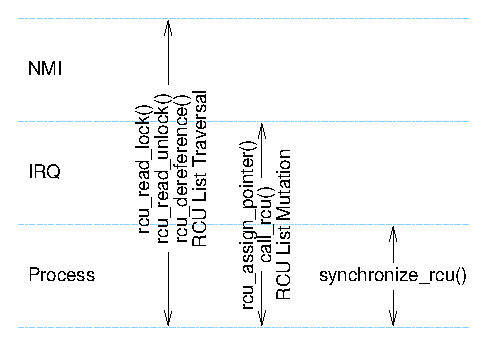
\includegraphics{defer/RCUenvAPI}}
\end{center}
\caption{RCU API Usage Constraints}
\label{fig:defer:RCU API Usage Constraints}
\end{figure}

Figure~\ref{fig:defer:RCU API Usage Constraints}
shows which APIs may be used in which in-kernel environments.
The RCU read-side primitives may be used in any environment, including NMI,
the RCU mutation and asynchronous grace-period primitives may be used in any
environment other than NMI, and, finally, the RCU synchronous grace-period
primitives may be used only in process context.
The RCU list-traversal primitives include \url{list_for_each_entry_rcu()},
\url{hlist_for_each_entry_rcu()}, etc.
Similarly, the RCU list-mutation primitives include
\url{list_add_rcu()}, \url{hlist_del_rcu()}, etc.

Note that primitives from other families of RCU may be substituted,
for example, \url{srcu_read_lock()} may be used in any context
in which \url{rcu_read_lock()} may be used.

\subsubsection{So, What \emph{is} RCU Really?}
\label{sec:defer:So, What is RCU Really?}

At its core, RCU is nothing more nor less than an API that supports
publication and subscription for insertions, waiting for all RCU readers
to complete, and maintenance of multiple versions.
That said, it is possible to build higher-level constructs
on top of RCU, including the reader-writer-locking, reference-counting,
and existence-guarantee constructs listed in the companion article.
Furthermore, I have no doubt that the Linux community will continue to
find interesting new uses for RCU,
just as they do for any of a number of synchronization
primitives throughout the kernel.

Of course, a more-complete view of RCU would also include
all of the things you can do with these APIs.

However, for many people, a complete view of RCU must include sample
RCU implementations.
The next section therefore presents a series of ``toy'' RCU implementations
of increasing complexity and capability.
